% Options for packages loaded elsewhere
\PassOptionsToPackage{unicode}{hyperref}
\PassOptionsToPackage{hyphens}{url}
\PassOptionsToPackage{dvipsnames,svgnames*,x11names*}{xcolor}
%
\documentclass[
  ignorenonframetext,
]{beamer}
\usepackage{pgfpages}
\setbeamertemplate{caption}[numbered]
\setbeamertemplate{caption label separator}{: }
\setbeamercolor{caption name}{fg=normal text.fg}
\beamertemplatenavigationsymbolsempty
% Prevent slide breaks in the middle of a paragraph
\widowpenalties 1 10000
\raggedbottom
\setbeamertemplate{part page}{
  \centering
  \begin{beamercolorbox}[sep=16pt,center]{part title}
    \usebeamerfont{part title}\insertpart\par
  \end{beamercolorbox}
}
\setbeamertemplate{section page}{
  \centering
  \begin{beamercolorbox}[sep=12pt,center]{part title}
    \usebeamerfont{section title}\insertsection\par
  \end{beamercolorbox}
}
\setbeamertemplate{subsection page}{
  \centering
  \begin{beamercolorbox}[sep=8pt,center]{part title}
    \usebeamerfont{subsection title}\insertsubsection\par
  \end{beamercolorbox}
}
\AtBeginPart{
  \frame{\partpage}
}
\AtBeginSection{
  \ifbibliography
  \else
    \frame{\sectionpage}
  \fi
}
\AtBeginSubsection{
  \frame{\subsectionpage}
}
\usepackage{lmodern}
\usepackage{amssymb,amsmath}
\usepackage{ifxetex,ifluatex}
\ifnum 0\ifxetex 1\fi\ifluatex 1\fi=0 % if pdftex
  \usepackage[T1]{fontenc}
  \usepackage[utf8]{inputenc}
  \usepackage{textcomp} % provide euro and other symbols
\else % if luatex or xetex
  \usepackage{unicode-math}
  \defaultfontfeatures{Scale=MatchLowercase}
  \defaultfontfeatures[\rmfamily]{Ligatures=TeX,Scale=1}
\fi
% Use upquote if available, for straight quotes in verbatim environments
\IfFileExists{upquote.sty}{\usepackage{upquote}}{}
\IfFileExists{microtype.sty}{% use microtype if available
  \usepackage[]{microtype}
  \UseMicrotypeSet[protrusion]{basicmath} % disable protrusion for tt fonts
}{}
\makeatletter
\@ifundefined{KOMAClassName}{% if non-KOMA class
  \IfFileExists{parskip.sty}{%
    \usepackage{parskip}
  }{% else
    \setlength{\parindent}{0pt}
    \setlength{\parskip}{6pt plus 2pt minus 1pt}}
}{% if KOMA class
  \KOMAoptions{parskip=half}}
\makeatother
\usepackage{xcolor}
\IfFileExists{xurl.sty}{\usepackage{xurl}}{} % add URL line breaks if available
\IfFileExists{bookmark.sty}{\usepackage{bookmark}}{\usepackage{hyperref}}
\hypersetup{
  pdftitle={Population Assessment and Distance Sampling},
  pdfauthor={Zack Treisman},
  colorlinks=true,
  linkcolor=Maroon,
  filecolor=Maroon,
  citecolor=blue,
  urlcolor=Blue,
  pdfcreator={LaTeX via pandoc}}
\urlstyle{same} % disable monospaced font for URLs
\newif\ifbibliography
\usepackage{color}
\usepackage{fancyvrb}
\newcommand{\VerbBar}{|}
\newcommand{\VERB}{\Verb[commandchars=\\\{\}]}
\DefineVerbatimEnvironment{Highlighting}{Verbatim}{commandchars=\\\{\}}
% Add ',fontsize=\small' for more characters per line
\usepackage{framed}
\definecolor{shadecolor}{RGB}{248,248,248}
\newenvironment{Shaded}{\begin{snugshade}}{\end{snugshade}}
\newcommand{\AlertTok}[1]{\textcolor[rgb]{0.94,0.16,0.16}{#1}}
\newcommand{\AnnotationTok}[1]{\textcolor[rgb]{0.56,0.35,0.01}{\textbf{\textit{#1}}}}
\newcommand{\AttributeTok}[1]{\textcolor[rgb]{0.77,0.63,0.00}{#1}}
\newcommand{\BaseNTok}[1]{\textcolor[rgb]{0.00,0.00,0.81}{#1}}
\newcommand{\BuiltInTok}[1]{#1}
\newcommand{\CharTok}[1]{\textcolor[rgb]{0.31,0.60,0.02}{#1}}
\newcommand{\CommentTok}[1]{\textcolor[rgb]{0.56,0.35,0.01}{\textit{#1}}}
\newcommand{\CommentVarTok}[1]{\textcolor[rgb]{0.56,0.35,0.01}{\textbf{\textit{#1}}}}
\newcommand{\ConstantTok}[1]{\textcolor[rgb]{0.00,0.00,0.00}{#1}}
\newcommand{\ControlFlowTok}[1]{\textcolor[rgb]{0.13,0.29,0.53}{\textbf{#1}}}
\newcommand{\DataTypeTok}[1]{\textcolor[rgb]{0.13,0.29,0.53}{#1}}
\newcommand{\DecValTok}[1]{\textcolor[rgb]{0.00,0.00,0.81}{#1}}
\newcommand{\DocumentationTok}[1]{\textcolor[rgb]{0.56,0.35,0.01}{\textbf{\textit{#1}}}}
\newcommand{\ErrorTok}[1]{\textcolor[rgb]{0.64,0.00,0.00}{\textbf{#1}}}
\newcommand{\ExtensionTok}[1]{#1}
\newcommand{\FloatTok}[1]{\textcolor[rgb]{0.00,0.00,0.81}{#1}}
\newcommand{\FunctionTok}[1]{\textcolor[rgb]{0.00,0.00,0.00}{#1}}
\newcommand{\ImportTok}[1]{#1}
\newcommand{\InformationTok}[1]{\textcolor[rgb]{0.56,0.35,0.01}{\textbf{\textit{#1}}}}
\newcommand{\KeywordTok}[1]{\textcolor[rgb]{0.13,0.29,0.53}{\textbf{#1}}}
\newcommand{\NormalTok}[1]{#1}
\newcommand{\OperatorTok}[1]{\textcolor[rgb]{0.81,0.36,0.00}{\textbf{#1}}}
\newcommand{\OtherTok}[1]{\textcolor[rgb]{0.56,0.35,0.01}{#1}}
\newcommand{\PreprocessorTok}[1]{\textcolor[rgb]{0.56,0.35,0.01}{\textit{#1}}}
\newcommand{\RegionMarkerTok}[1]{#1}
\newcommand{\SpecialCharTok}[1]{\textcolor[rgb]{0.00,0.00,0.00}{#1}}
\newcommand{\SpecialStringTok}[1]{\textcolor[rgb]{0.31,0.60,0.02}{#1}}
\newcommand{\StringTok}[1]{\textcolor[rgb]{0.31,0.60,0.02}{#1}}
\newcommand{\VariableTok}[1]{\textcolor[rgb]{0.00,0.00,0.00}{#1}}
\newcommand{\VerbatimStringTok}[1]{\textcolor[rgb]{0.31,0.60,0.02}{#1}}
\newcommand{\WarningTok}[1]{\textcolor[rgb]{0.56,0.35,0.01}{\textbf{\textit{#1}}}}
\usepackage{graphicx,grffile}
\makeatletter
\def\maxwidth{\ifdim\Gin@nat@width>\linewidth\linewidth\else\Gin@nat@width\fi}
\def\maxheight{\ifdim\Gin@nat@height>\textheight\textheight\else\Gin@nat@height\fi}
\makeatother
% Scale images if necessary, so that they will not overflow the page
% margins by default, and it is still possible to overwrite the defaults
% using explicit options in \includegraphics[width, height, ...]{}
\setkeys{Gin}{width=\maxwidth,height=\maxheight,keepaspectratio}
% Set default figure placement to htbp
\makeatletter
\def\fps@figure{htbp}
\makeatother
\setlength{\emergencystretch}{3em} % prevent overfull lines
\providecommand{\tightlist}{%
  \setlength{\itemsep}{0pt}\setlength{\parskip}{0pt}}
\setcounter{secnumdepth}{-\maxdimen} % remove section numbering

\pgfdeclareimage[width=3.5cm]{mcslogo}{../western_logo_hor_MCS_3C_pos.pdf}
\pgfdeclareimage[width=1cm]{ccbysa}{../ccbysa88x31.png}
\titlegraphic{\href{http://creativecommons.org/licenses/by-sa/4.0/}{\pgfuseimage{ccbysa}}
\hfill
\href{https://western.edu/program/mathematics/}{\pgfuseimage{mcslogo}}}
%\usecolortheme{wcu}
%\institute{Western Colorado University}
%\setbeamertemplate{navigation symbols}{}

\title{Population Assessment and Distance Sampling}
\author{Zack Treisman}
\date{Spring 2021}

\begin{document}
\frame{\titlepage}

\begin{frame}{Philosophy}
\protect\hypertarget{philosophy}{}

Wildlife population assessment - \emph{How many are there?}

\end{frame}

\begin{frame}{Simpler questions:}
\protect\hypertarget{simpler-questions}{}

\begin{itemize}
\tightlist
\item
  rank
\item
  occupancy
\item
  index
\end{itemize}

\end{frame}

\begin{frame}{Population}
\protect\hypertarget{population}{}

\begin{itemize}
\tightlist
\item
  census
\item
  mark-recapture
\item
  removal
\item
  plot sampling
\item
  distance sampling
\end{itemize}

\end{frame}

\begin{frame}[fragile]{A simulated example}
\protect\hypertarget{a-simulated-example}{}

We'll use some of the code from the section on simulation to generate
random arrangements of populations.

\scriptsize

\begin{Shaded}
\begin{Highlighting}[]
\NormalTok{pos <-}\StringTok{ }\KeywordTok{random_pop}\NormalTok{()}
\end{Highlighting}
\end{Shaded}

\normalsize

The simulated population size is 458. \scriptsize

\begin{Shaded}
\begin{Highlighting}[]
\KeywordTok{ggplot}\NormalTok{(}\DataTypeTok{data=}\NormalTok{pos, }\KeywordTok{aes}\NormalTok{(offspr_x, offspr_y))}\OperatorTok{+}\KeywordTok{geom_point}\NormalTok{()}\OperatorTok{+}\KeywordTok{labs}\NormalTok{(}\DataTypeTok{x=}\StringTok{""}\NormalTok{, }\DataTypeTok{y=}\StringTok{""}\NormalTok{)}
\end{Highlighting}
\end{Shaded}

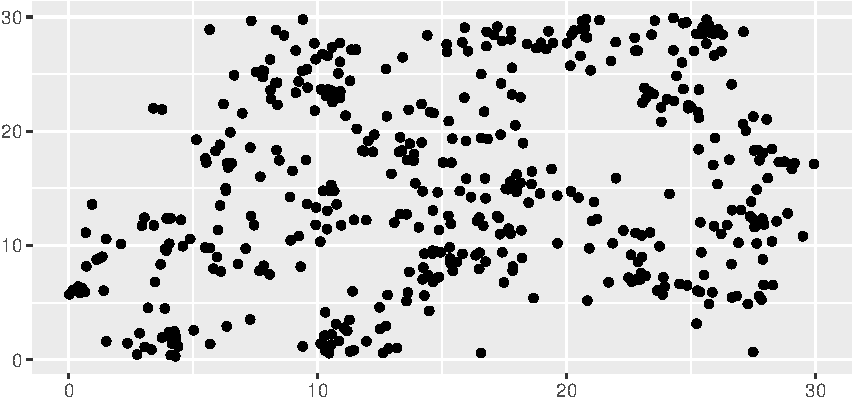
\includegraphics{distance_sampling_files/figure-beamer/unnamed-chunk-4-1.pdf}

\end{frame}

\begin{frame}[fragile]{Capture-mark-recapture}
\protect\hypertarget{capture-mark-recapture}{}

\begin{itemize}
\tightlist
\item
  Capture a subset of the population and mark them.
\item
  Release. After sufficient time for the released subset to have fully
  mixed with the population, capture another subset.
\item
  The fraction of the second capture that is marked estimates the
  fraction of the population in the first capture.
\item
  As a formula: \(\hat P = C_1/p_m\) where

  \begin{itemize}
  \tightlist
  \item
    \(\hat P\) is the population estimate,
  \item
    \(C_1\) is the size of the first captured group and
  \item
    \(p_m\) is the marked proportion in the second captured group.
  \end{itemize}
\end{itemize}

\scriptsize

\begin{Shaded}
\begin{Highlighting}[]
\NormalTok{capture1 <-}\StringTok{ }\KeywordTok{sample}\NormalTok{(}\KeywordTok{nrow}\NormalTok{(pos), }\DecValTok{50}\NormalTok{) }
\NormalTok{pos}\OperatorTok{$}\NormalTok{mark <-}\StringTok{ }\DecValTok{1}\OperatorTok{:}\KeywordTok{nrow}\NormalTok{(pos) }\OperatorTok\StringTok{ }\NormalTok{capture1}

\NormalTok{capture2 <-}\StringTok{  }\KeywordTok{sample}\NormalTok{(}\KeywordTok{nrow}\NormalTok{(pos), }\DecValTok{50}\NormalTok{)}
\NormalTok{pos}\OperatorTok{$}\NormalTok{recapture <-}\StringTok{ }\NormalTok{(}\DecValTok{1}\OperatorTok{:}\KeywordTok{nrow}\NormalTok{(pos) }\OperatorTok\StringTok{ }\NormalTok{capture2) }\OperatorTok{&}\StringTok{ }\NormalTok{pos}\OperatorTok{$}\NormalTok{mark}
\end{Highlighting}
\end{Shaded}

\normalsize

\begin{itemize}
\tightlist
\item
  There are 7 recaptures.
\item
  This is 0.14 of the second captured group.
\item
  The population estimate is 50/0.14=357.
\end{itemize}

\end{frame}

\begin{frame}[fragile]{Plot of captures and recaptures}
\protect\hypertarget{plot-of-captures-and-recaptures}{}

This method is not particularly well suited to populations that don't
move around and mingle.

\scriptsize

\begin{Shaded}
\begin{Highlighting}[]
\KeywordTok{ggplot}\NormalTok{(}\DataTypeTok{data=}\NormalTok{pos, }\KeywordTok{aes}\NormalTok{(offspr_x, offspr_y, }\DataTypeTok{color=}\NormalTok{mark, }\DataTypeTok{shape=}\NormalTok{recapture))}\OperatorTok{+}
\StringTok{  }\KeywordTok{geom_point}\NormalTok{()}\OperatorTok{+}\KeywordTok{labs}\NormalTok{(}\DataTypeTok{x=}\StringTok{""}\NormalTok{, }\DataTypeTok{y=}\StringTok{""}\NormalTok{)}
\end{Highlighting}
\end{Shaded}

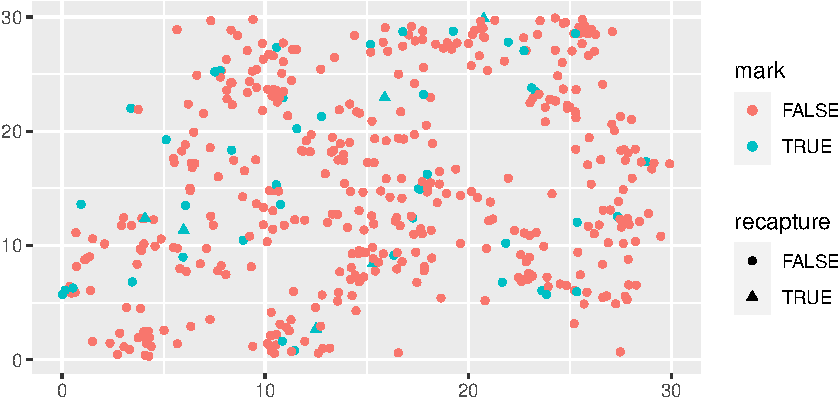
\includegraphics{distance_sampling_files/figure-beamer/unnamed-chunk-6-1.pdf}

\end{frame}

\begin{frame}{Capture-mark-recapture is fundamentally Bayesian}
\protect\hypertarget{capture-mark-recapture-is-fundamentally-bayesian}{}

Population estimates can be improved over time by repeating the
experiment.

\end{frame}

\begin{frame}{Plot Sampling}
\protect\hypertarget{plot-sampling}{}

Even if the individuals being counted don't move around, it is often
impractical/unreasonable/impossible to census an entire area of
interest. Instead, we often census appropriately chosen subplots.

\begin{itemize}
\tightlist
\item
  Subplots are often laid out along transects.
\end{itemize}

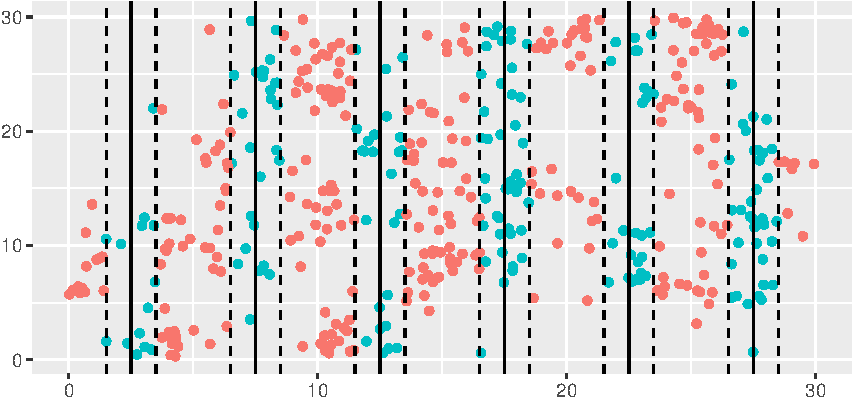
\includegraphics{distance_sampling_files/figure-beamer/unnamed-chunk-7-1.pdf}

\end{frame}

\begin{frame}[fragile]{Computing population from plot sampling}
\protect\hypertarget{computing-population-from-plot-sampling}{}

Divide the number counted in the plots by the fraction of the area that
is covered by the plots.

\scriptsize

\begin{Shaded}
\begin{Highlighting}[]
\NormalTok{num_plots <-}\StringTok{ }\DecValTok{5}
\NormalTok{half_width <-}\StringTok{ }\DecValTok{1}
\NormalTok{Lx <-}\StringTok{ }\DecValTok{30}\NormalTok{; Ly <-}\StringTok{ }\DecValTok{30}
\NormalTok{counted <-}\StringTok{ }\KeywordTok{sum}\NormalTok{(pos}\OperatorTok{$}\NormalTok{in_plot)}
\NormalTok{area_plots <-}\StringTok{ }\NormalTok{Ly}\OperatorTok{*}\DecValTok{2}\OperatorTok{*}\NormalTok{half_width}\OperatorTok{*}\NormalTok{num_plots}
\NormalTok{total_area <-}\StringTok{ }\NormalTok{Lx}\OperatorTok{*}\NormalTok{Ly}
\NormalTok{area_fraction <-}\StringTok{ }\NormalTok{area_plots}\OperatorTok{/}\NormalTok{total_area}
\NormalTok{(pop_estimate <-}\StringTok{ }\NormalTok{counted}\OperatorTok{/}\NormalTok{area_fraction)}
\end{Highlighting}
\end{Shaded}

\begin{verbatim}
## [1] 528
\end{verbatim}

\normalsize

We can use a bootstrap to get a confidence interval for this estimate.

\end{frame}

\begin{frame}[fragile]{Distance sampling}
\protect\hypertarget{distance-sampling}{}

What if detecting the individuals in the population is challenging?

\begin{itemize}
\tightlist
\item
  In many surveys, the further the individual is from the observer, the
  lower the probability of observation.
\end{itemize}

\scriptsize

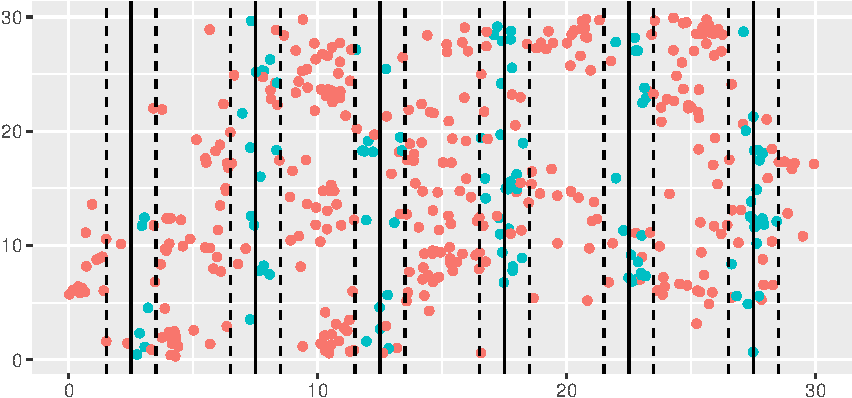
\includegraphics{distance_sampling_files/figure-beamer/unnamed-chunk-10-1.pdf}

\begin{Shaded}
\begin{Highlighting}[]
\NormalTok{counted <-}\StringTok{ }\KeywordTok{sum}\NormalTok{(pos}\OperatorTok{$}\NormalTok{detected)}
\NormalTok{(pop_estimate <-}\StringTok{ }\NormalTok{counted}\OperatorTok{/}\NormalTok{area_fraction)}
\end{Highlighting}
\end{Shaded}

\begin{verbatim}
## [1] 309
\end{verbatim}

\end{frame}

\begin{frame}{Overall detection probability}
\protect\hypertarget{overall-detection-probability}{}

It is useful to look at a histogram of the distance of detected
individuals.

\begin{itemize}
\tightlist
\item
  Goal: fit a detection probability function to these data.
\end{itemize}

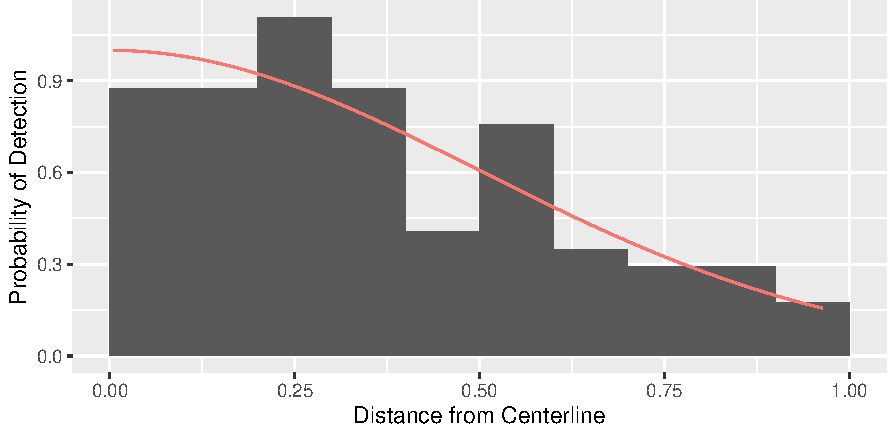
\includegraphics{distance_sampling_files/figure-beamer/unnamed-chunk-12-1.pdf}
The overall probability of detection is \(\hat P=\) 0.5981.

\end{frame}

\begin{frame}[fragile]{Estimation using \(\hat P\)}
\protect\hypertarget{estimation-using-hat-p}{}

To get an estimated count from a count where the probability of
detection is not 100\%, divide the actual count by the overall
probability of detection.

\scriptsize

\begin{Shaded}
\begin{Highlighting}[]
\NormalTok{est_count <-}\StringTok{ }\NormalTok{counted}\OperatorTok{/}\NormalTok{overall_prob}
\NormalTok{(pop_estimate <-}\StringTok{ }\NormalTok{est_count}\OperatorTok{/}\NormalTok{area_fraction)}
\end{Highlighting}
\end{Shaded}

\begin{verbatim}
## [1] 516.598
\end{verbatim}

\end{frame}

\begin{frame}[fragile]{Guessing the detection probability function}
\protect\hypertarget{guessing-the-detection-probability-function}{}

We have some data that we would like to use to define a curve.

\begin{itemize}
\tightlist
\item
  Propose a shape for the detection probability function (half-normal,
  hazard rate, uniform, \ldots).

  \begin{itemize}
  \tightlist
  \item
    \(p_{det}(0)=1\) (objects at the centerline are detected)
  \item
    \(p'_{det}(0)=0\) (detection probability is rather flat around 0)
  \item
    \(p'_{det}(x)\leq0\) (detection probability decreases with distance)
  \end{itemize}
\item
  Use maximum likelihood to find parameters of the most appropriate
  curve in the family.
\end{itemize}

The \(\hat P\) above comes from rescaling a normal distribution with
\(\sigma=0.5\) so that \(p_{det}(0)=1\). The choice of \(\sigma\) was
from fitting by eye. The code below finds the \(\sigma\) for the maximum
likelihood. \scriptsize

\begin{Shaded}
\begin{Highlighting}[]
\NormalTok{samp_ind<-pos[pos}\OperatorTok{$}\NormalTok{in_plot,]}
\NormalTok{prob_detect2 <-}\StringTok{ }\ControlFlowTok{function}\NormalTok{(x,s) }\KeywordTok{dnorm}\NormalTok{(x,}\DataTypeTok{sd=}\NormalTok{s)}\OperatorTok{/}\KeywordTok{dnorm}\NormalTok{(}\DecValTok{0}\NormalTok{, }\DataTypeTok{sd=}\NormalTok{s)}
\NormalTok{nll_fn<-}\ControlFlowTok{function}\NormalTok{(s) }\OperatorTok{-}\KeywordTok{sum}\NormalTok{(}\KeywordTok{dbinom}\NormalTok{(samp_ind}\OperatorTok{$}\NormalTok{detected,}
                                \DecValTok{1}\NormalTok{,}\KeywordTok{prob_detect2}\NormalTok{(samp_ind}\OperatorTok{$}\NormalTok{d,s),}
                                \DataTypeTok{log =} \OtherTok{TRUE}\NormalTok{))}
\NormalTok{opt1 <-}\StringTok{ }\KeywordTok{optim}\NormalTok{(}\DataTypeTok{fn =}\NormalTok{ nll_fn, }\DataTypeTok{par =} \KeywordTok{list}\NormalTok{(}\DataTypeTok{s=}\FloatTok{0.5}\NormalTok{), }\DataTypeTok{method=}\StringTok{"BFGS"}\NormalTok{); opt1}\OperatorTok{$}\NormalTok{par}
\end{Highlighting}
\end{Shaded}

\begin{verbatim}
##         s 
## 0.4852794
\end{verbatim}

\end{frame}

\begin{frame}[fragile]{Using the optimal half-normal detection
probability}
\protect\hypertarget{using-the-optimal-half-normal-detection-probability}{}

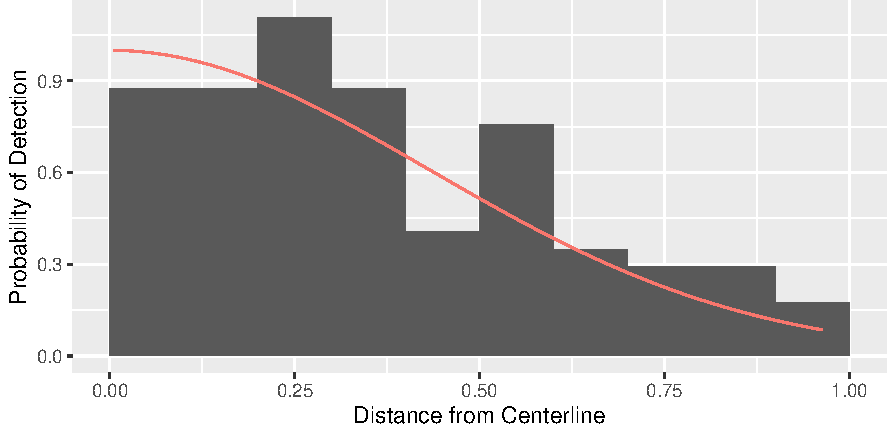
\includegraphics{distance_sampling_files/figure-beamer/unnamed-chunk-15-1.pdf}

\scriptsize

\begin{Shaded}
\begin{Highlighting}[]
\NormalTok{overall_prob2 <-}\StringTok{ }\KeywordTok{integrate}\NormalTok{(}\ControlFlowTok{function}\NormalTok{(x) }\KeywordTok{prob_detect2}\NormalTok{(x,}\DataTypeTok{s=}\NormalTok{opt1}\OperatorTok{$}\NormalTok{par),}\DecValTok{0}\NormalTok{,}\DecValTok{1}\NormalTok{)}\OperatorTok{$}\NormalTok{value }
\NormalTok{est_count2 <-}\StringTok{ }\NormalTok{counted}\OperatorTok{/}\NormalTok{overall_prob2}
\NormalTok{(pop_estimate2 <-}\StringTok{ }\NormalTok{est_count2}\OperatorTok{/}\NormalTok{area_fraction)}
\end{Highlighting}
\end{Shaded}

\begin{verbatim}
## [1] 528.8525
\end{verbatim}

\end{frame}

\begin{frame}{Hazard rate detection probaility functions.}
\protect\hypertarget{hazard-rate-detection-probaility-functions.}{}

A half-normal detection probability function may not be best.

The hazard rate detection probability is defined by \[
p_{det}(x)=1-\exp(-(x/\sigma)^{-b}).
\] This function has two parameters, \(\sigma\) which controls the width
of the shoulder, and \(b\) which controls the steepness of the dropoff.

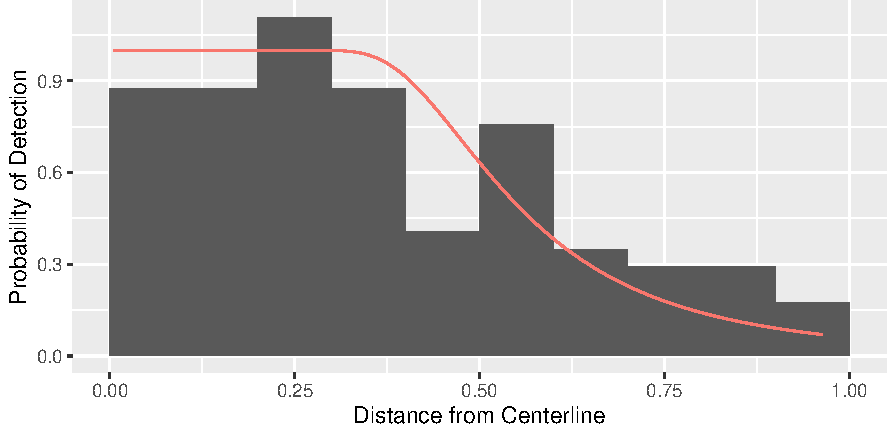
\includegraphics{distance_sampling_files/figure-beamer/unnamed-chunk-17-1.pdf}

\end{frame}

\begin{frame}[fragile]{Maximum likelihood to find the optimal hazard
rate}
\protect\hypertarget{maximum-likelihood-to-find-the-optimal-hazard-rate}{}

Again, we can use maximum likelihood to estimate the parameters.

\scriptsize

\begin{Shaded}
\begin{Highlighting}[]
\NormalTok{prob_detect_hr <-}\StringTok{ }\ControlFlowTok{function}\NormalTok{(x,s,b) }\DecValTok{1}\OperatorTok{-}\KeywordTok{exp}\NormalTok{(}\OperatorTok{-}\NormalTok{(x}\OperatorTok{/}\NormalTok{s)}\OperatorTok{^}\NormalTok{(}\OperatorTok{-}\NormalTok{b))}
\NormalTok{nll_fn_hr <-}\StringTok{ }\ControlFlowTok{function}\NormalTok{(pars)\{s<-pars[}\DecValTok{1}\NormalTok{];b<-pars[}\DecValTok{2}\NormalTok{]}
\OperatorTok{-}\KeywordTok{sum}\NormalTok{(}\KeywordTok{dbinom}\NormalTok{(samp_ind}\OperatorTok{$}\NormalTok{detected,}\DecValTok{1}\NormalTok{,}\KeywordTok{prob_detect_hr}\NormalTok{(samp_ind}\OperatorTok{$}\NormalTok{d,s,b), }\DataTypeTok{log =} \OtherTok{TRUE}\NormalTok{))\}}
\NormalTok{opt2 <-}\StringTok{ }\KeywordTok{optim}\NormalTok{(}\DataTypeTok{fn =}\NormalTok{ nll_fn_hr, }\DataTypeTok{par =} \KeywordTok{list}\NormalTok{(}\DataTypeTok{s=}\FloatTok{0.25}\NormalTok{, }\DataTypeTok{b=}\DecValTok{4}\NormalTok{)); opt2}\OperatorTok{$}\NormalTok{par}
\end{Highlighting}
\end{Shaded}

\begin{verbatim}
##         s         b 
## 0.3546658 1.0210627
\end{verbatim}

\end{frame}

\begin{frame}{The optimal Hazard Rate detection curve}
\protect\hypertarget{the-optimal-hazard-rate-detection-curve}{}

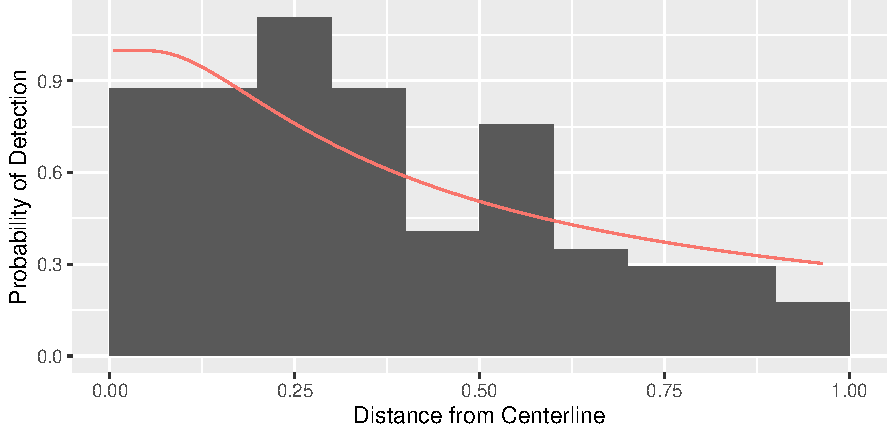
\includegraphics{distance_sampling_files/figure-beamer/unnamed-chunk-19-1.pdf}

\end{frame}

\begin{frame}[fragile]{Using the optimal Hazard Rate function to predict
\(\hat P\)}
\protect\hypertarget{using-the-optimal-hazard-rate-function-to-predict-hat-p}{}

And then we estimate

\begin{itemize}
\tightlist
\item
  the overall probability \(\hat P\) by integrating the detection
  probability function,
\item
  the number of individuals within the sampling region by dividing the
  count by \(\hat P\), and
\item
  the population by dividing the number of individuals by the area
  fraction.
\end{itemize}

\scriptsize

\begin{Shaded}
\begin{Highlighting}[]
\NormalTok{overall_prob3<-}\KeywordTok{integrate}\NormalTok{(}\ControlFlowTok{function}\NormalTok{(x)\{}
  \KeywordTok{prob_detect_hr}\NormalTok{(x,}\DataTypeTok{s=}\NormalTok{opt2}\OperatorTok{$}\NormalTok{par[}\DecValTok{1}\NormalTok{],}\DataTypeTok{b=}\NormalTok{opt2}\OperatorTok{$}\NormalTok{par[}\DecValTok{2}\NormalTok{])\},}\DecValTok{0}\NormalTok{,}\DecValTok{1}\NormalTok{)}\OperatorTok{$}\NormalTok{value  }
\NormalTok{est_count3 <-}\StringTok{ }\NormalTok{counted}\OperatorTok{/}\NormalTok{overall_prob3}
\NormalTok{(pop_estimate3 <-}\StringTok{ }\NormalTok{est_count3}\OperatorTok{/}\NormalTok{area_fraction)}
\end{Highlighting}
\end{Shaded}

\begin{verbatim}
## [1] 537.1223
\end{verbatim}

\end{frame}

\begin{frame}{Assumptions and issues}
\protect\hypertarget{assumptions-and-issues}{}

\begin{itemize}
\item
  If the individuals that are being counted are clustered (pods of
  whales, clusters of plants, \ldots), this can cause problems.

  \begin{itemize}
  \tightlist
  \item
    Estimate the distance to the center of the cluster.
  \item
    Record the size of each cluster and estimate the mean cluster size.
  \end{itemize}
\item
  Often, instead of using all observations, it makes sense to truncate
  observations above some effecting strip width.
\item
  If there is avoidance of the observer, this can cause problems.
\end{itemize}

\end{frame}

\begin{frame}{Point-transect distance sampling}
\protect\hypertarget{point-transect-distance-sampling}{}

For studies where the observer is stationary, the process is quite
similar.

\end{frame}

\begin{frame}{References}
\protect\hypertarget{references}{}

\end{frame}

\end{document}
